\cotefile{156-4}
\scanpage{50}
\mspage{49}

\deleted{\uline{Cont 5} If $F$ and $G$ are two disjoint figures, and \unsure{if} $F'$, \deleted{$G'$\illegible{1} of} subdivision\unsure{s|{}}\unsure{,} \inserted{of $F$} then $F'$ and $G$ are disjoint.} \margin{\deleted{[\uline{NB} $F'\cap G$ is defined as, it is $F'$ and $G$ \uline{compatible} that is at issue.}}

\deleted{\uline{Corollary} If $F'$ refines $F$, $G'$ refines $G$, \deleted{then} $F$ and $G$ disjoint then $F'$ and $G'$ disjoint.}

\margin{\begin{tikzpicture}[x=.5cm,y=.5cm]\draw(0,0)--(0,1.5);\draw(.13,0)--(.13,1.5);\end{tikzpicture}}\uline{C\deleted{\unsure{ont|ompt|onst}} 5} Let $F$ be a figure, $F'$ a subdivision of $F$. \deleted{\unsure{A}}Then for every figure $G$, $G$ is disjoint ; $F$ if and only if it is disjoint\unsure{e} from $F'$

\uline{NB} It suffices to postulate it for elementary $G$.

It then follows from \deleted{\uline{Cont 4}} C4 that $F'\cup G$ is a subdivision of $F\cup G$.

\uline{Corollary} Let $F$ and $G$ be disjoint figures, then for $F'\ll F$, $G'\ll F$, $F'$ and $G'$ are disjoint, and $F'\cup G'\ll F\cup G$. If $F'$ and $G'$ are subdivisions of $F,G$, then $F'\cup G'$ is one of $F\cup G$.

\margin{\begin{tikzpicture}[x=.5cm,y=.5cm]\draw(0,0)--(0,1.5);\draw(.13,0)--(.13,1.5);\end{tikzpicture}}\uline{C 6} (Induced subdivisions) Let $F$ be a figure, $F'$ a subdivision of $F$, $G$ a subfigure of $F$. Then there exists a unique subdivision $G'$ of $G$, such that
\[G'\subset F'\]
(induced subdivision) \inserted{and $G'$ is formed of the $X\in F'$ such that $X\ll G$}
\figure{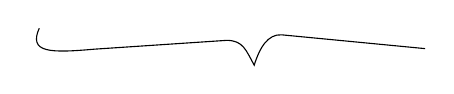
\begin{tikzpicture}[x=1cm,y=1cm,scale=.7]
\draw (0,.25)..controls(-.2,-.2)and(.2,-.2)..(1,-.13)--(3.4,.03)..controls(3.7,.03)and(3.75,-.15)..(3.9,-.42)..controls(4,-.1)and(4.15,.15)..(4.4,.13)--(7,-.12);
\end{tikzpicture}}

\margin{NB \inserted{Double} Transitivity of induction. \uline{Notation} $F'|G$}

\margin{\begin{tikzpicture}[x=.5cm,y=.5cm]\draw(0,0)--(0,1.5);\draw(.13,0)--(.13,1.5);\end{tikzpicture}}\uline{C 7} (\deleted{\unsure{D|R}}Gluing of subdivisions) Let $F$ be a figure, \deleted{\unsure{each} \illegible{3} every} \inserted{$F_i$ subfigures} \deleted{$X\in$} such that $F=\bigcup F_i$. Let, for every $i$, $F'_i$ be a subdivision of $F_i$, and suppose
